%%%%%%%%%%%%%%%%%%%%%%%%%%%%%%%%%%%%%%%%%%%%%%%%%%%%%%%%%
%%
%%					PAPER CONFIG
%%
%%					This configures the paper environment.
%%					The biggest thing is to set the root directory appropriately.
%%%%%%%%%%%%%%%%%%%%%%%%%%%%%%%%%%%%%%%%%%%%%%%%%%%%%%%
%%
\newcommand*{\RootDirectory}{"/Users/Mark/Documents/UW/Research/H5+/paper"}

%%%%%%%%%%%%%%%%%%%%%%%%%%%%%%%%%%%%%%%%%%%%%%%%%%%%%%%%%%%%%%%%%%%%%
%% This is a (brief) model paper using the achemso class
%% The document class accepts keyval options, which should include
%% the target journal and optionally the manuscript type.
%%%%%%%%%%%%%%%%%%%%%%%%%%%%%%%%%%%%%%%%%%%%%%%%%%%%%%%%%%%%%%%%%%%%%
\documentclass[journal=jacsat, manuscript=article, layout=twocolumn]{achemso}

%%%%%%%%%%%%%%%%%%%%%%%%%%%%%%%%%%%%%%%%%%%%%%%%%%%%%%%%%%%%%%%%%%%%%
%% If issues arise when submitting your manuscript, you may want to
%% un-comment the next line.  This provides information on the
%% version of every file you have used.
%%%%%%%%%%%%%%%%%%%%%%%%%%%%%%%%%%%%%%%%%%%%%%%%%%%%%%%%%%%%%%%%%%%%%
% \listfiles

\usepackage{import}

\import{\RootDirectory}{config/packages.tex}

\import{\RootDirectory}{config/custom.tex}

\import{\RootDirectory}{config/author.tex}

\import{\RootDirectory}{config/title.tex}

\import{\RootDirectory}{config/keywords.tex}

%\begin{document}

%%%%%%%%%%%%%%%%%%%%%%%%%%%%%%%%%%%%%%%%%%%%%%%%
%%
%%                                   SI FIGURES
%%%%%%%%%%%%%%%%%%%%%%%%%%%%%%%%%%%%%%%%%%%%%%%%
%%
\newpage
%%%%%%%%%%%%%%%%%%%%%%%%%%%%%
%%%%%%%%%%%%%%%%%%%
%%BIG FIGS
\begin{figure}[ht]
\begin{center}
    \includegraphics[width=0.9\textwidth]{\RootDirectory/figures/adiabats.pdf}
    \caption{
    \reffig{adiabat_cuts} but scaled up so the differences are easier to see
}
\label{fig:adiabat_cuts_big}
\end{center}
\end{figure}


%%%%%%%%%%%%%%%%%%%%%%%%%%%%%%%%%%%%%%%%%%%%%%%%
%%  SPECTRA
\begin{figure}[ht]
\begin{center}
    \includegraphics[width=0.9\textwidth]{\RootDirectory/figures/spec_chunk_1.pdf}
    \caption{
    Comparison of our results (red) with prior theoretical work out of our group~\cite{Lin2012} (blue) and priori experimental work~\cite{Cheng2012} (green). Note the general red shift of our results relative to prior theory. Owing to nature of the experiment the experimental intensities will not agree with our work, particularly at low energies, but the general pattern is good. The frequency blue shift relative to experiment, however, suggests a need to refine the grid of the calculation. \CHECK
}
\label{fig:spec_chunk_1}
\end{center}
\end{figure}

\begin{figure}[ht]
\begin{center}
    \includegraphics[width=0.9\textwidth]{\RootDirectory/figures/spec_chunk_2.pdf}
    \caption{
    Comparison of our results (red) with prior theoretical work out of our group~\cite{Lin2012} (blue) and priori experimental work~\cite{Cheng2012} (green). The large peaks are where the \hplus{} progression building off a single quantum in the \htwo{} vibrations begins. Note the good agreement in pattern.
}
\label{fig:spec_chunk_2}
\end{center}
\end{figure}

\begin{figure}[ht]
\begin{center}
    \includegraphics[width=0.9\textwidth]{\RootDirectory/figures/spec_chunk_3.pdf}
    \caption{
    Comparison of our results (red) with unpublished experimental work out of the Duncan group (green). The general pattern is suggestive and the lack of intensity in transitions beyond $6000$ \wavenumbers{} indicates that we will need to introduce two quanta of \htwo{} excitation to reproduce these results.
}
\label{fig:spec_chunk_3}
\end{center}
\end{figure}

\begin{figure}[ht]
\begin{center}
    \includegraphics[width=0.9\textwidth]{\RootDirectory/figures/zhou_comp.pdf}
    \caption{
    Figures \ref{fig:spec_chunk_1}, \ref{fig:spec_chunk_2}, and \ref{fig:spec_chunk_3} spliced together into one figure. Note that the relative intensities of the experimental spectra is unknown, so they were normalized to the height of the dominant peak coming out of theory in each portion.
}
\label{fig:zhou_comp}
\end{center}
\end{figure}

\begin{figure}[ht]
\begin{center}
    \includegraphics[width=0.9\textwidth]{\RootDirectory/figures/no_coupling.pdf}
    \caption{
    Figures \ref{fig:spec_chunk_2} and \ref{fig:spec_chunk_3} but comparing our results with coupling (red) to our results without coupling (blue)
}
\label{fig:no_coupling}
\end{center}
\end{figure}

\begin{figure}[ht]
\begin{center}
    \includegraphics[width=0.9\textwidth]{\RootDirectory/figures/no_coupling_higher.pdf}
    \caption{
    \reffig{no_coupling} but focused solely on the frequency range in \reffig{spec_chunk_3}
}
\label{fig:no_coupling_higher}
\end{center}
\end{figure}

%%%%%%%%%%%%%%%%%%%%%%%%%%%%%%%%%%%%%%%%%%%%%%%%
%%  WAVEFUNCTIONS
%%
\begin{figure}[ht]
\begin{center}
    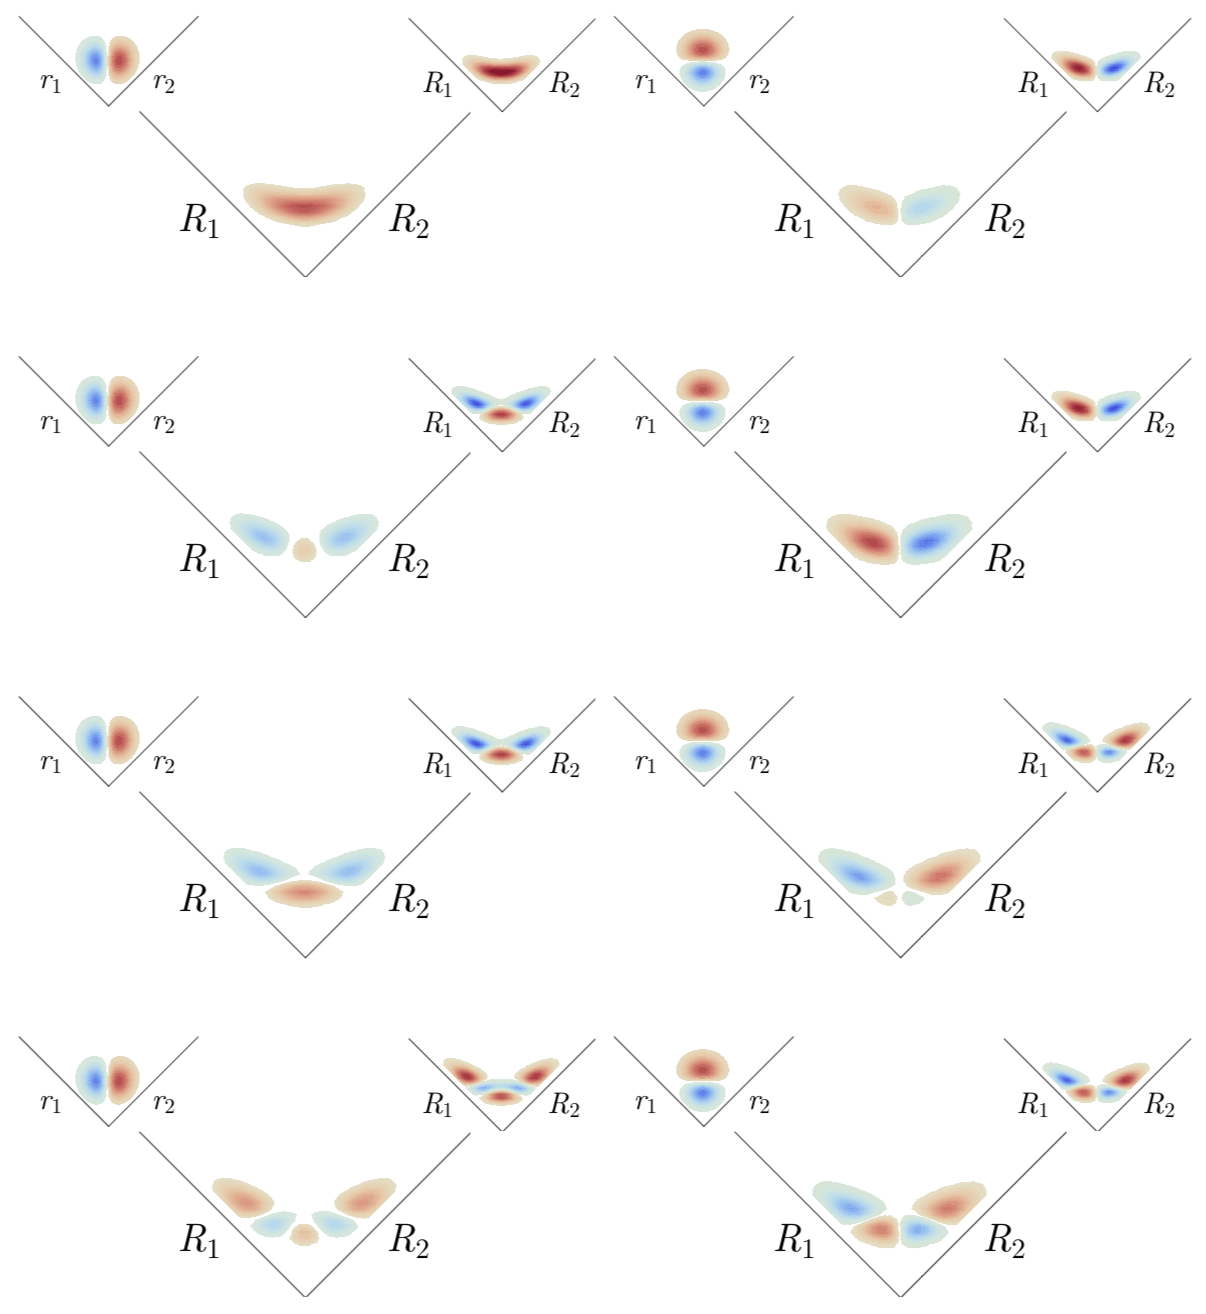
\includegraphics[width=0.9\textwidth]{\RootDirectory/figures/wavefunctions_grid_1.png}
    \caption{
    The projections of the first four states with significant intensity coming out of the coupled calculation, corresponding to the peaks at 3370 \wavenumbers{}, 3863 \wavenumbers{}, 4133 \wavenumbers{}, and 4503 \wavenumbers{}. \LOL  Each row shows the two projection states with the projection onto the lower energy adiabat on the left and the projection onto the higher energy adiabat on the right with each labeled by its \htwo{} wavefunction in the top left and the dominant \hplus{} wavefunction in the top right. Note that each state, when multiplied by its \htwo{} state, is antisymmetric and can thus carry intensity }
\label{fig:wavefunctions_grid_1}
\end{center}
\end{figure}

\begin{figure}[ht]
\begin{center}
    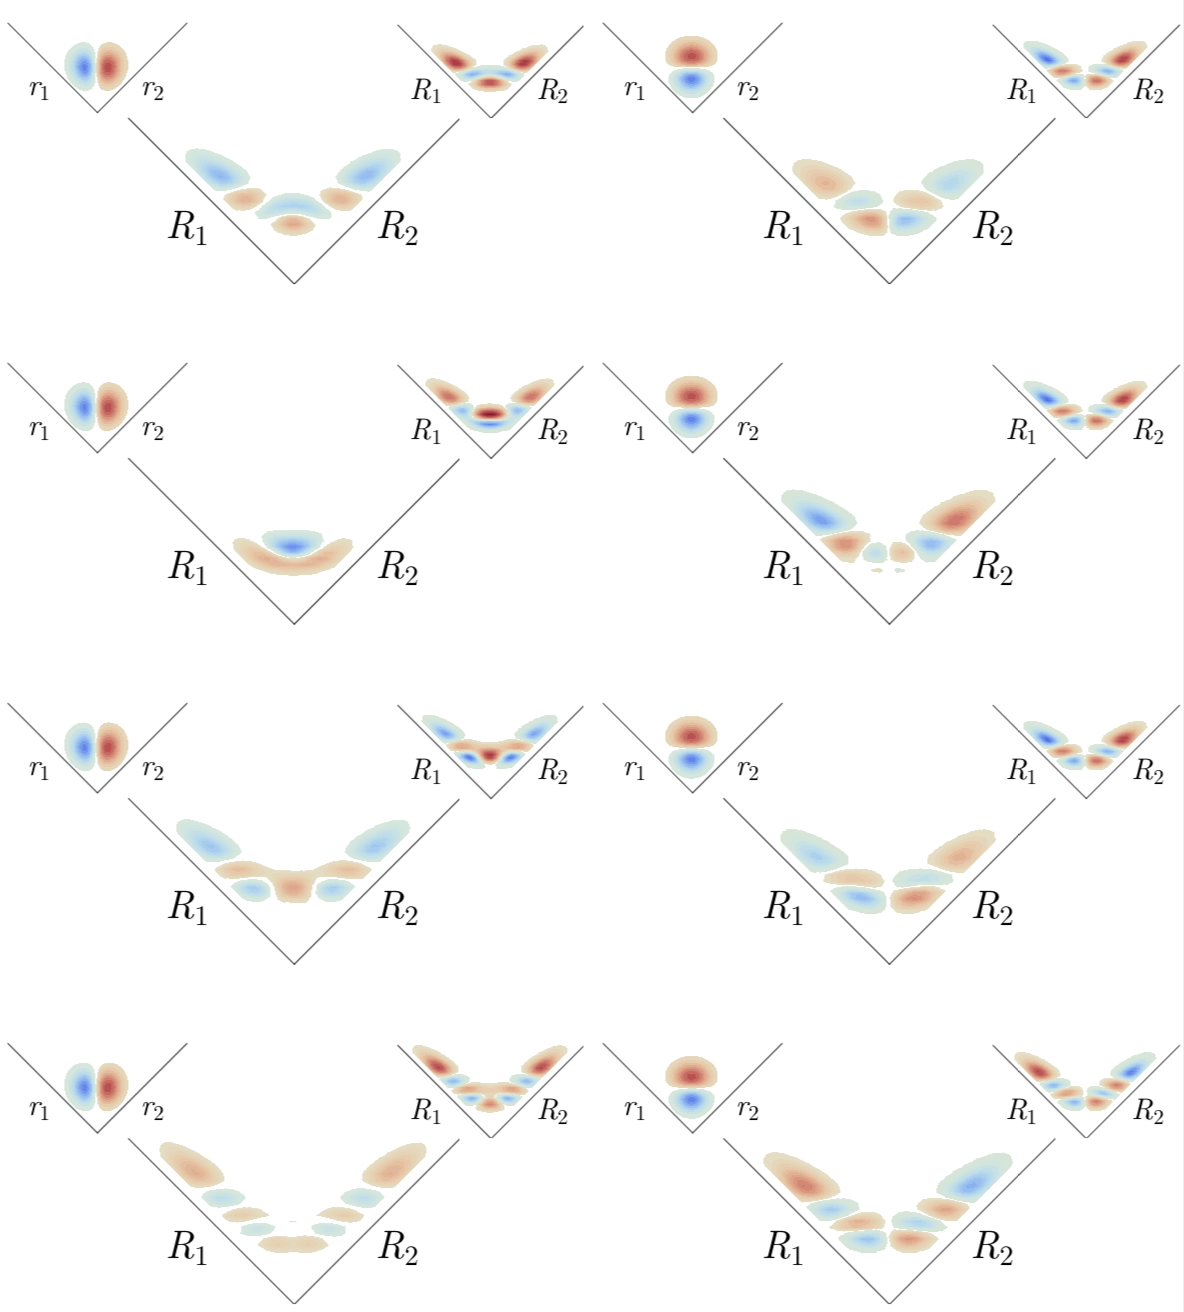
\includegraphics[width=0.9\textwidth]{\RootDirectory/figures/wavefunctions_grid_2.png}
    \caption{ The same as Figure \ref{fig:wavefunctions_grid_1} but for the the peaks at 4999 \wavenumbers{}, 5139 \wavenumbers{}, and 5281 \wavenumbers{}}
\label{fig:wavefunctions_grid_2}
\end{center}
\end{figure}

%\end{document}
